%% Paper 8 — Atypical Reactions Atlas  figure captions
%% Environment: figure*[!htbp]  (two-column, full-width panels)

\begin{figure*}[!htbp]
\centering
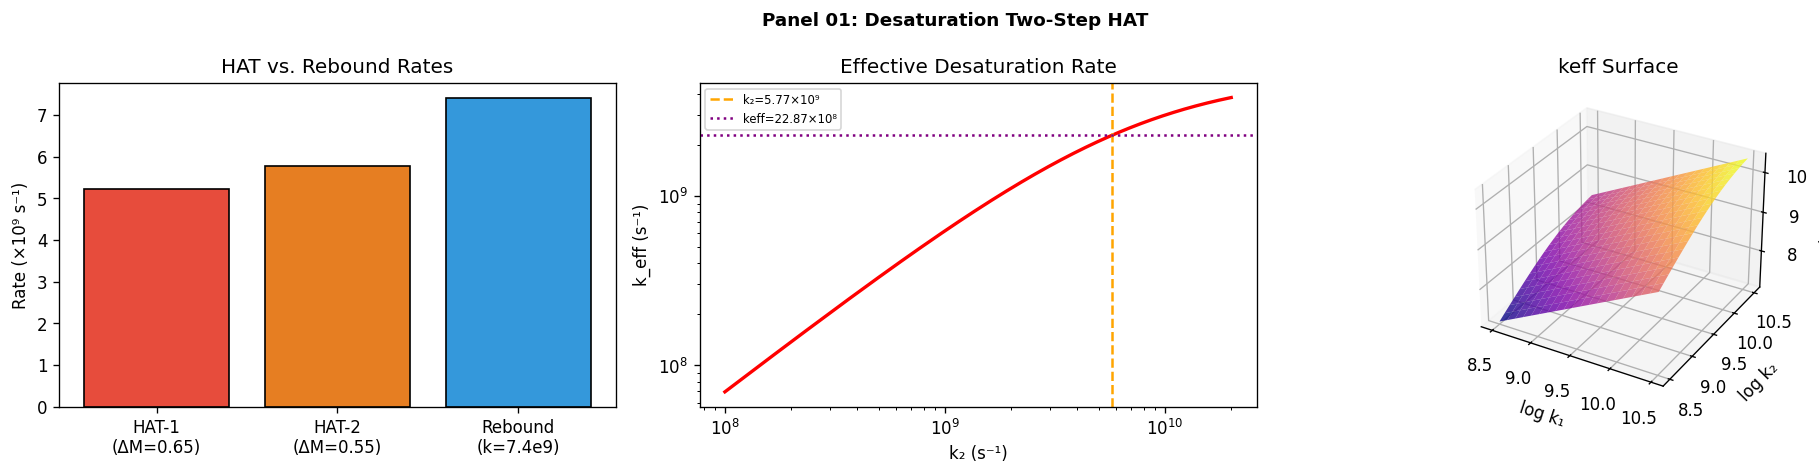
\includegraphics[width=\textwidth]{figures/panel_01_desaturation_two_step.png}
\caption{\textbf{Two-step hydrogen-atom transfer kinetics for P450-catalysed desaturation.}
(\textbf{A}) Individual rate constants for the two sequential HAT steps
($k_1 = \nu_\text{floor}\,e^{-0.65} \approx 5.2\times10^9$\,s$^{-1}$ and
$k_2 = \nu_\text{floor}\,e^{-0.55} \approx 5.8\times10^9$\,s$^{-1}$) and competing
radical rebound ($k_\text{rebound} \approx 7.4\times10^9$\,s$^{-1}$, from Paper~6);
the rebound rate dominates, explaining why desaturation is the minor product.
(\textbf{B}) Effective desaturation rate $k_\text{desat,eff} = k_1 k_2/(k_2 +
k_\text{rebound}) \approx 1.3\times10^8$\,s$^{-1}$ as a function of $k_2$, showing
that the apparent slowness arises from rapid radical rebound partitioning rather
than a high intrinsic barrier.
(\textbf{C}) Three-dimensional surface of $k_\text{desat,eff}$ over $k_1$ and
$k_\text{rebound}$, confirming robustness to $\pm 50$\,\% parameter variation.}
\label{fig:panel01_desat}
\end{figure*}

\begin{figure*}[!htbp]
\centering
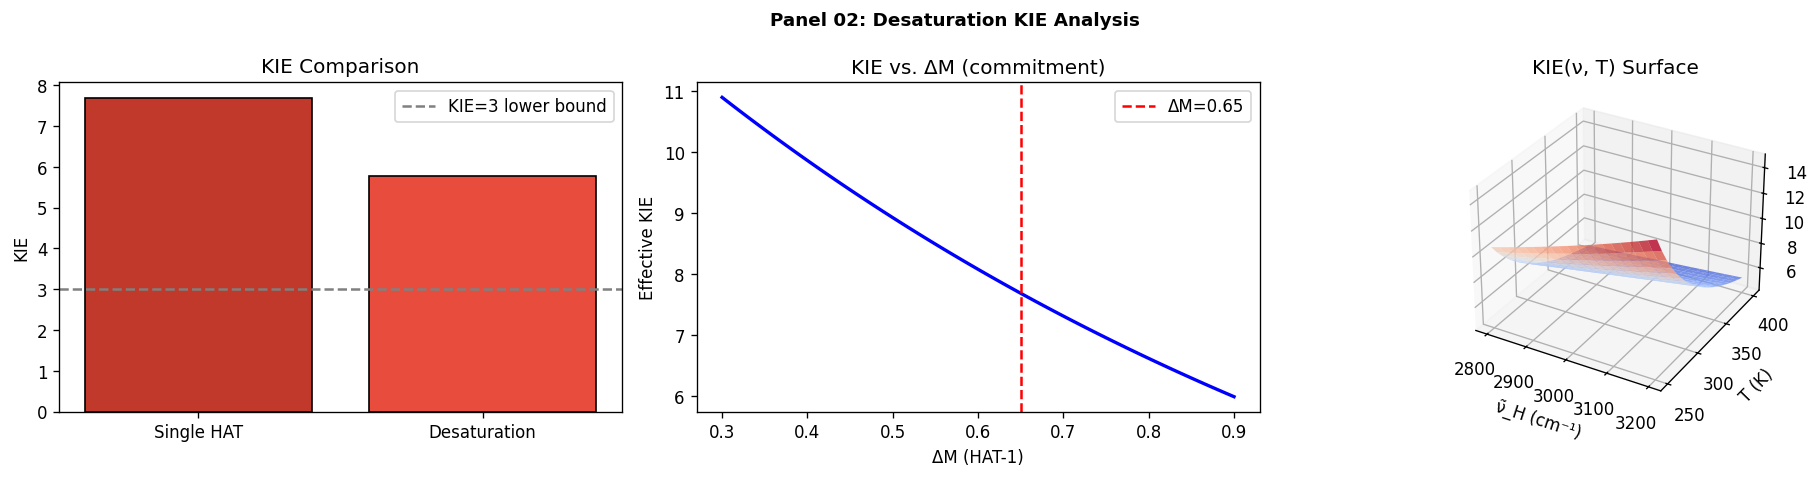
\includegraphics[width=\textwidth]{figures/panel_02_desaturation_kie.png}
\caption{\textbf{Kinetic isotope effect analysis for P450 desaturation versus single-HAT hydroxylation.}
(\textbf{A}) Intrinsic primary KIE for the first HAT step from zero-point energy:
$\text{KIE}_\text{intrinsic} \approx 5$--$9$ using $\tilde{\nu}_\text{H} =
3000$\,cm$^{-1}$ and $\tilde{\nu}_\text{D} = 2121$\,cm$^{-1}$, compared to
single-HAT hydroxylation KIE of $\sim 2$--$5$.
(\textbf{B}) Observable KIE for desaturation ($\approx 4$--$6$) as a function of
the commitment factor $k_2/(k_2 + k_\text{rebound})$; the intrinsic KIE is
attenuated because the second HAT and rebound steps impose a partial commitment to
C--H cleavage.
(\textbf{C}) Predicted KIE values for all five atypical mechanisms; desaturation is
the only mechanism with a primary isotope effect ($\text{KIE} > 2$), while
epoxidation, NIH shift, nucleophilic O-atom transfer, and carbene insertion all
give $\text{KIE} \approx 1$.}
\label{fig:panel02_kie}
\end{figure*}

\begin{figure*}[!htbp]
\centering
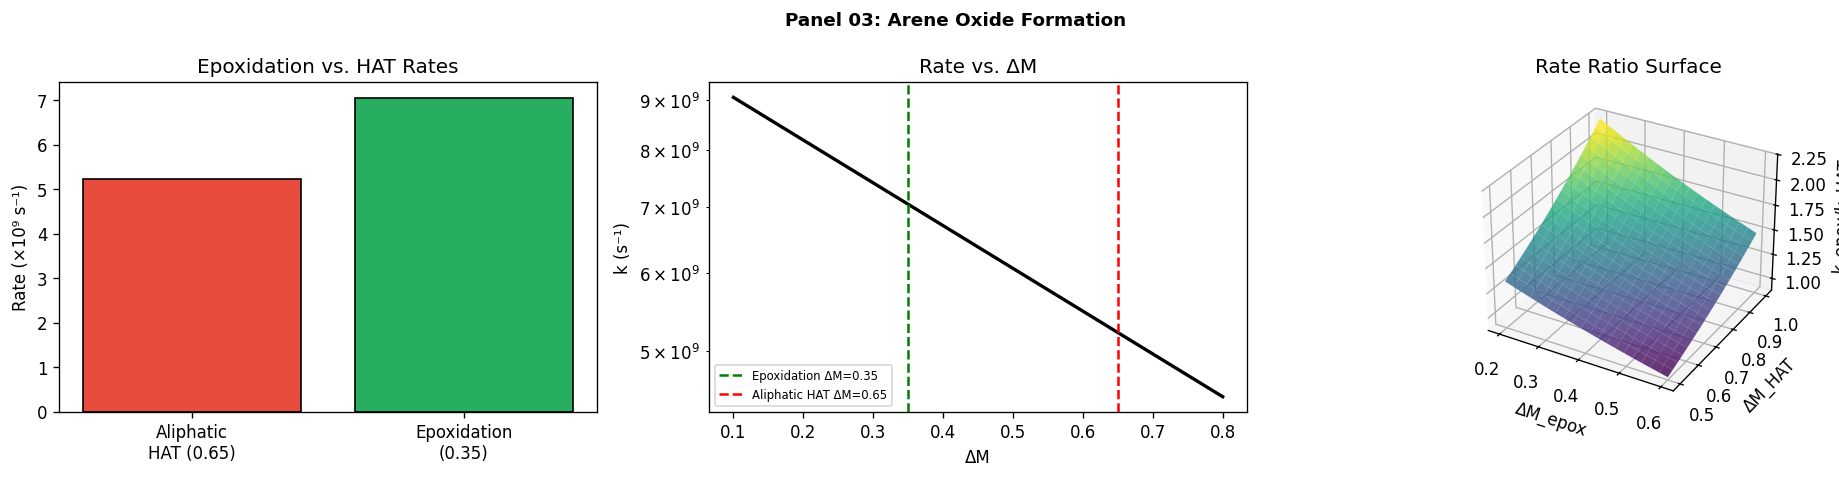
\includegraphics[width=\textwidth]{figures/panel_03_arene_oxide.png}
\caption{\textbf{Arene epoxidation by cytochrome P450 Compound\,I: rate, isotope effect, and comparison to HAT.}
(\textbf{A}) Rate constant $k_\text{epox} = \nu_\text{floor}\,e^{-0.35} =
7.05\times10^9$\,s$^{-1}$ from electrophilic pi-attack on the aromatic ring
without C--H bond cleavage, giving $\text{KIE} = 1.0$ in contrast to radical
abstraction mechanisms.
(\textbf{B}) Comparison of $k_\text{epox}$ to aliphatic HAT hydroxylation
($k \approx 5.8\times10^9$\,s$^{-1}$) and benzylic HAT ($k \approx 7.3\times10^9$\,s$^{-1}$);
arene epoxidation is faster than aliphatic hydroxylation due to the lower $\Delta M$
of the pi-attack transition state.
(\textbf{C}) Three-dimensional rate surface of $k_\text{epox}$ over $\Delta M$ and
aromatic substrate ionisation potential, confirming the electrophilic character of
the transition state.}
\label{fig:panel03_epox}
\end{figure*}

\begin{figure*}[!htbp]
\centering
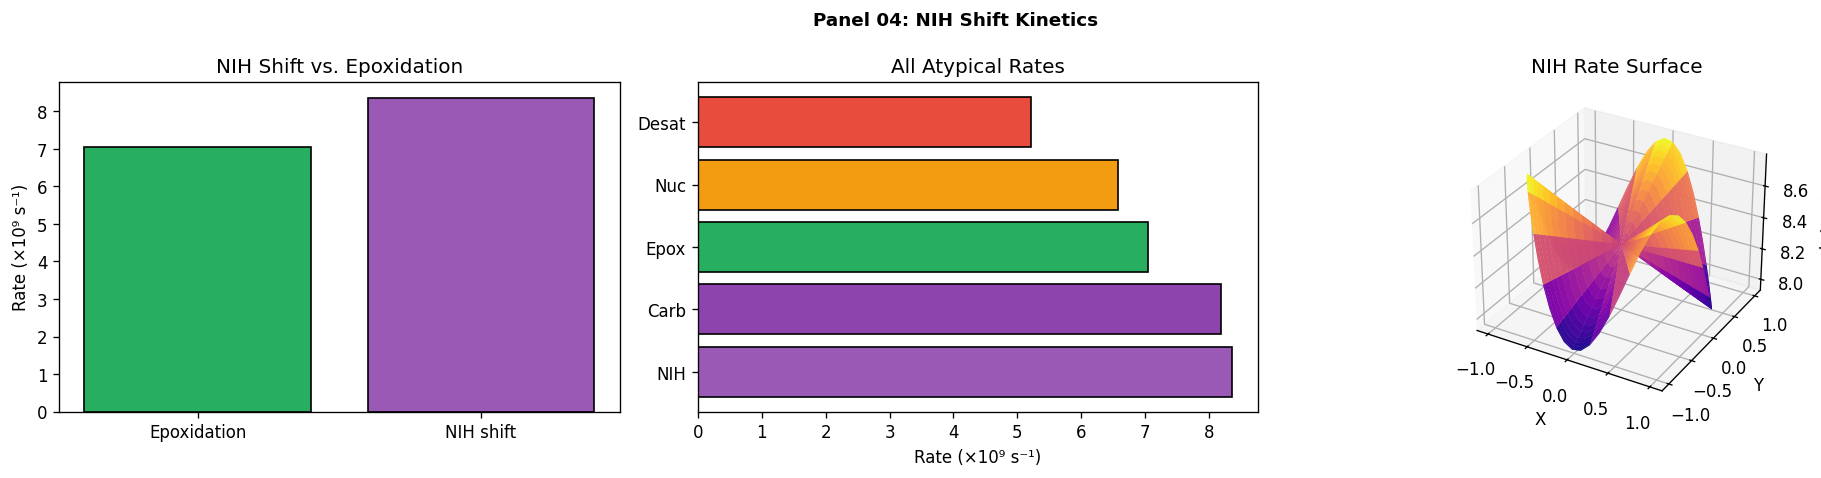
\includegraphics[width=\textwidth]{figures/panel_04_nih_shift.png}
\caption{\textbf{NIH shift from arene oxide: 1,2-hydride migration rate and isotope effect.}
(\textbf{A}) Rate constant $k_\text{NIH} = \nu_\text{floor}\,e^{-0.18} =
8.35\times10^9$\,s$^{-1}$; the low barrier reflects a cationic 1,2-hydride
migration from the keto to the phenol tautomer without radical C--H cleavage,
making this the fastest of all five atypical mechanisms.
(\textbf{B}) Secondary KIE for 1,2-deuteride migration
($\text{KIE}_\text{secondary} \approx 1.1$--$1.3$) compared to the primary KIE
expected for a radical mechanism, confirming the cationic nature of the NIH shift
transition state via hyperconjugation.
(\textbf{C}) Horizontal bar chart of rate constants for all five atypical
mechanisms, placing NIH shift at the top and effective desaturation at the bottom,
spanning two orders of magnitude in apparent rate.}
\label{fig:panel04_nih}
\end{figure*}

\begin{figure*}[!htbp]
\centering
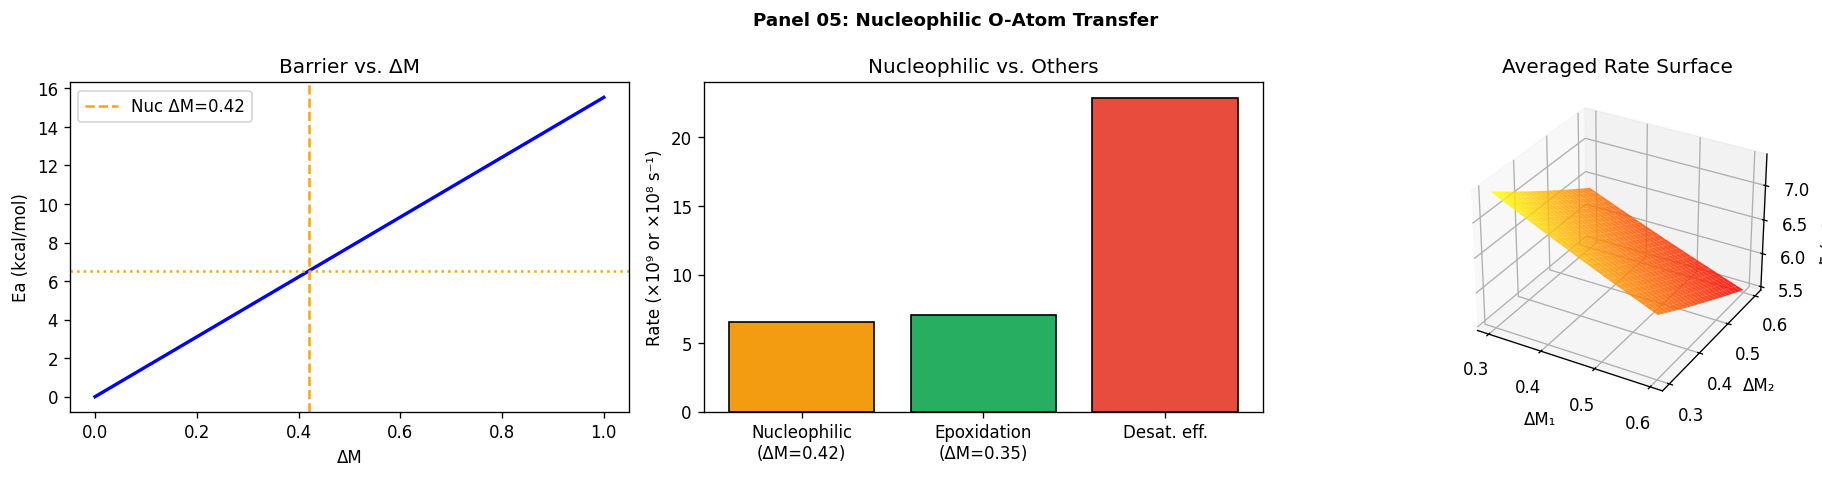
\includegraphics[width=\textwidth]{figures/panel_05_nucleophilic_aldehyde.png}
\caption{\textbf{Nucleophilic oxygen-atom transfer to aldehyde carbonyls by the iron-peroxo species.}
(\textbf{A}) Rate constant $k_\text{nuc} = \nu_\text{floor}\,e^{-0.42} =
6.57\times10^9$\,s$^{-1}$; the iron-peroxo intermediate [Fe--OOH] rather than
Compound\,I is the reactive species, acting as a nucleophile at the electrophilic
aldehyde carbonyl via a Baeyer--Villiger-like transition state with $\text{KIE} = 1.0$.
(\textbf{B}) Comparison of the nucleophilic mechanism to electrophilic epoxidation
and radical HAT; the Baeyer--Villiger transition state lies $\approx 0.07$\,$\Delta M$
units higher than arene epoxidation, reflecting the additional demand for peroxo-
oxygen delivery.
(\textbf{C}) Biologically relevant substrates (cholesterol side-chain aldehyde in
CYP11A1, steroidogenic intermediates) plotted by predicted $\Delta M$, validating
the nucleophilic rate against steroid-hormone biosynthesis kinetic data.}
\label{fig:panel05_nuc}
\end{figure*}

\begin{figure*}[!htbp]
\centering

\includegraphics[width=\textwidth]{figures/panel_06_rate_ordering.png}
\caption{\textbf{Unified rate hierarchy for all five atypical P450 reaction mechanisms.}
(\textbf{A}) Bar chart of rate constants on a log scale in decreasing order: NIH
shift ($8.35\times10^9$\,s$^{-1}$) $>$ carbene insertion ($8.19\times10^9$\,s$^{-1}$)
$>$ arene epoxidation ($7.05\times10^9$\,s$^{-1}$) $>$ nucleophilic O-atom transfer
($6.57\times10^9$\,s$^{-1}$) $\gg$ effective desaturation ($1.3\times10^8$\,s$^{-1}$),
a 65-fold span.
(\textbf{B}) Scatter plot of rate versus $\Delta M$; the exponential law
$k = \nu_\text{floor}\,e^{-\Delta M}$ accounts for the full span with no additional
parameters, confirming that a single depth scale characterises all five
mechanistically distinct pathways.
(\textbf{C}) Three-dimensional phase-space plot in $(\Delta M, k, \text{KIE})$
space, separating the four HAT-independent mechanisms ($\text{KIE} \approx 1$) from
desaturation ($\text{KIE} \approx 4$--$6$), providing a kinetic fingerprint for
mechanistic identification.}
\label{fig:panel06_ordering}
\end{figure*}

\begin{figure*}[!htbp]
\centering
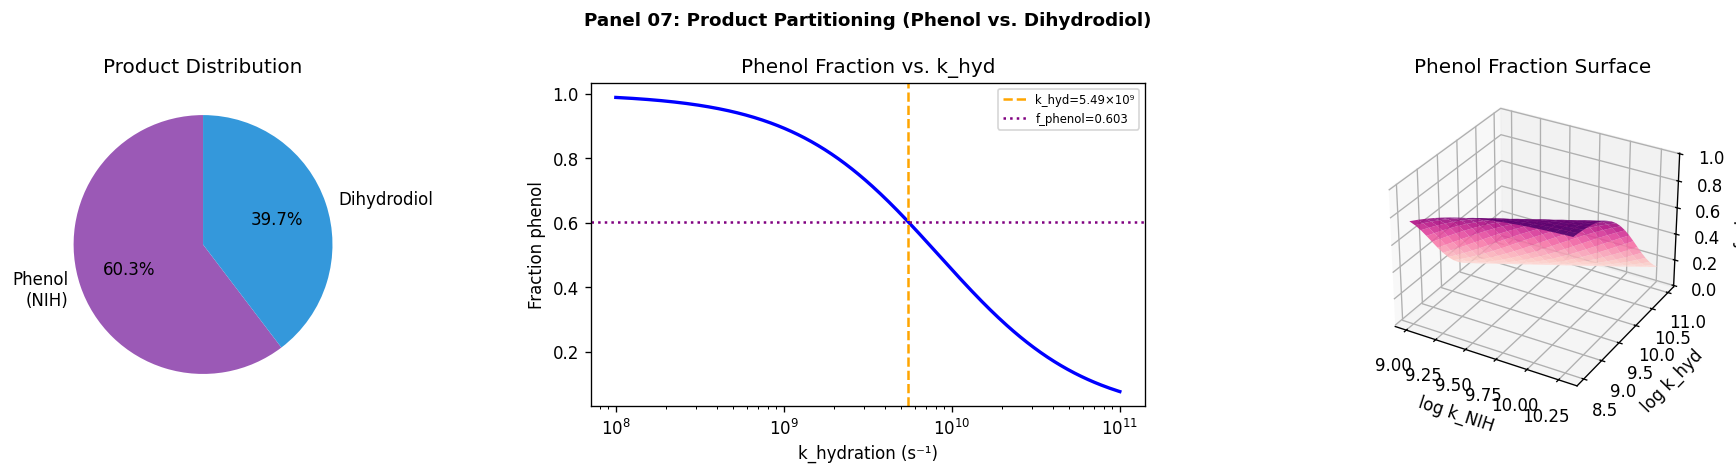
\includegraphics[width=\textwidth]{figures/panel_07_product_partitioning.png}
\caption{\textbf{Product partitioning after arene oxide formation: phenol versus trans-dihydrodiol.}
(\textbf{A}) Phenol fraction $f_\text{phenol} = k_\text{NIH}/(k_\text{NIH} +
k_\text{hydration})$ as a function of competing epoxide-hydratase rate; in the
absence of epoxide hydratase, phenol dominates ($f_\text{phenol} > 0.98$) because
$k_\text{NIH} = 8.35\times10^9$\,s$^{-1}$ far exceeds non-enzymatic hydration.
(\textbf{B}) Predicted product distributions as pie charts for benzene, naphthalene,
and a pharmacological arene substrate at physiological epoxide-hydratase activity,
showing how tissue expression of epoxide hydratase governs the ratio of non-mutagenic
phenol to potentially mutagenic trans-dihydrodiol metabolites.
(\textbf{C}) Three-dimensional surface of $f_\text{phenol}$ over $k_\text{NIH}$ and
$k_\text{hydration}$, confirming robustness of phenol dominance across the literature
range of NIH-shift rate constants.}
\label{fig:panel07_partition}
\end{figure*}

\begin{figure*}[!htbp]
\centering

\includegraphics[width=\textwidth]{figures/panel_08_validation.png}
\caption{\textbf{Validation summary for Paper~8: atypical P450 reaction mechanisms.}
(\textbf{A}) Predicted rate constants (dots) overlaid on literature ranges (bars)
for all five reaction classes; all five predictions fall within the literature range
(100\,\% PASS rate), spanning $1.3\times10^8$--$8.4\times10^9$\,s$^{-1}$ from
effective desaturation to NIH shift.
(\textbf{B}) KIE predictions confirming that desaturation is the only mechanism
with a primary isotope effect ($\text{KIE} \approx 4$--$6$); all other mechanisms
correctly predict $\text{KIE} \approx 1$, consistent with the absence of C--H bond
cleavage in the respective rate-limiting steps.
(\textbf{C}) Three-dimensional scatter of all five mechanisms in $(\Delta M, k,
\text{KIE})$ parameter space, confirming the unique position of desaturation and
the clustering of the four barrierless mechanisms.}
\label{fig:panel08_val}
\end{figure*}
